%%%%%%%%%%%%%%%%%%%%%%%%%%%%%%%%%%%%%%%%%%%%%%%%%%%%%%%%%%%%%%%%
%%%%%%%%%%%%%%%%%%%%%%%%%%%%%%%%%%%%%%%%%%%%%%%%%%%%%%%%%%%%%%%%
%%%%
%%%% This text file is part of the source of 
%%%% `Introduction to High-Performance Scientific Computing'
%%%% by Victor Eijkhout, copyright 2012
%%%%
%%%% This book is distributed under a Creative Commons Attribution 3.0
%%%% Unported (CC BY 3.0) license and made possible by funding from
%%%% The Saylor Foundation \url{http://www.saylor.org}.
%%%%
%%%%
%%%%%%%%%%%%%%%%%%%%%%%%%%%%%%%%%%%%%%%%%%%%%%%%%%%%%%%%%%%%%%%%
%%%%%%%%%%%%%%%%%%%%%%%%%%%%%%%%%%%%%%%%%%%%%%%%%%%%%%%%%%%%%%%%

Let us take a look at the question `how much parallelism is there in a
program execution'. 
There is the theoretical question of the
absolutely maximum number of actions that can be taken in parallel,
but we also need to wonder what kind of actions these are and how hard
it is to actually execute them in parallel, as well has how efficient
the resulting execution is.

The discussion in this section will be mostly on a conceptual level;
in section~\ref{sec:parallel-programming} we will go into some detail
on how parallelism can actually be programmed.

\Level 1 {Data parallelism}
\label{sec:data-parallel}

It is fairly common for a program that have loops with a simple body,
that gets executed for all elements in a large data set:
\begin{verbatim}
for (i=0; i<1000000; i++)
  a[i] = 2*b[i];
\end{verbatim}
Such code is considered an instance of
\indextermsub{data}{parallelism} or
\indextermsub{fine-grained}{parallelism}. If you had as many
processors as array elements, this code would look very simple: each
processor would execute the statment
\begin{verbatim}
a = 2*b
\end{verbatim}
on its local data. 

If your code consists predominantly of such loops
over arrays, it can be executed efficiently with all processors in
lockstep. Architectures based on this idea, where the processors can
in fact \emph{only} work in lockstep, have existed, see
section~\ref{sec:simd}. Such fully parallel operations on arrays 
appear in computer graphics, where every pixel of an image is processed
independently. For this reason, \acp{GPU}
\begin{gpu}
  (section~\ref{sec:gpu})
\end{gpu}
are strongly based on data parallelism.

Continuing the above example for a little bit, consider the operation

\begin{displayalgorithm}
  \For{$0\leq i<\mathrm{max}$}{
    $i_{\mathrm{left}}=\mod(i-1,\mathrm{max})$\\
    $i_{\mathrm{right}}=\mod(i+1,\mathrm{max})$\\
    $a_i = (b_{i_{\mathrm{left}}}+b_{i_{\mathrm{right}}})/2$}
\end{displayalgorithm}

On a data parallel machine, that could be implemented as

\begin{displayalgorithm}
  \SetKw{shiftleft}{shiftleft}
  \SetKw{shiftright}{shiftright}
  $\n{bleft} \leftarrow \shiftright(\n{b})$\\
  $\n{bright} \leftarrow \shiftleft(\n{b})$\\
  $\n{a} \leftarrow (\n{bleft}+\n{bright})/2$
\end{displayalgorithm}

where the \n{shiftleft/right} instructions cause a data item to be
sent to the processor with a number lower or higher by~1.
%
For this second example to be efficient, it is necessary that each
processor can communicate quickly with its immediate neighbours, and
the first and last processor with each other. 

In
various contexts such a `blur' operations in graphics, it makes sense
to have operations on 2D data:

\begin{displayalgorithm}
  \For{$0<i<m$}{
    \For{$0<j<n$}{$a_{ij}\leftarrow (b_{ij-1}+b_{ij+1}+b_{i-1j}+b_{i+1j})$}}
\end{displayalgorithm}

and consequently processors have be able to move data to neighbours in
a 2D grid.

\Level 1 {Instruction-level parallelism}

In \indexac{ILP}, the parallelism is still on the level of individual
instructions, but these need not be similar. For instance, in 

\begin{displayalgorithm}
  $a\leftarrow b+c$\\ $d\leftarrow e*f$
\end{displayalgorithm}

the two assignments are independent, and can therefore be executed
simultaneously. This kind of parallelism is too cumbersome for humans
to identify, but \index{compiler}compilers are very good at this. In
fact, identifying \ac{ILP} is crucial for getting good performance out
of modern \indexterm{superscalar} CPUs.

\Level 1 {Task-level parallelism}
\label{sec:task-parallel}
\index{task!parallelism|(}

At the other extreme from data and instruction-level parallelism,
\emph{task parallelism} is about identifying whole subprograms
that can be executed in parallel. As an example, searching in a tree
data structure could be implemented as follows:

\begin{displayprocedure}{SearchInTree}{root}
  \SetKw{optimal}{optimal}\SetKw{exit}{exit}\SetKw{search}{SearchInTree}\SetKw{parl}{parallel}
  \eIf{\optimal(root)}{\exit}
  {\parl: \search(leftchild),\search(rightchild)}
\end{displayprocedure}

The search tasks in this example are not synchronized, and the number
of tasks is not fixed: it can grow arbitrarily. In practice, having
too many tasks is not a good idea, since processors are most efficient
if they work on just a single task. Tasks can then be scheduled as
follows:

\begin{displayalgorithm}
  \While{there are tasks left}{
    wait until a processor becomes inactive;\\
    spawn a new task on it}
\end{displayalgorithm}

(There is a subtle distinction between the two previous
pseudo-codes. In the first, tasks were self-scheduling: each task
spawned off two new ones. The second code is an example of
the \indexterm{master-worker paradigm}: there is one central task which
lives for the duration of the code, and which spawns and assigns the
worker tasks.)

Unlike in the data parallel example above, the assignment of data to
processor is not determined in advance in such a scheme. Therefore,
this mode of parallelism is most suited for thread-programming, for
instance through the OpenMP library; section~\ref{sec:openmp}.

Let us consider a more serious example of task-level parallelism.

A finite element mesh is, in the simplest case, a collection of
triangles that covers a 2D object. Since angles that are too acute
should be avoided, the \indexterm{Delauney mesh refinement} process
can take certain triangles, and replace them by better shaped
ones. This is illustrated in figure~\ref{fig:delauney}: the black
triangles violate some angle condition, so either they themselves get
subdivided, or they are joined with some neighbouring ones (rendered
in grey) and then jointly redivided.

\begin{figure}[ht]
    \begin{quote}
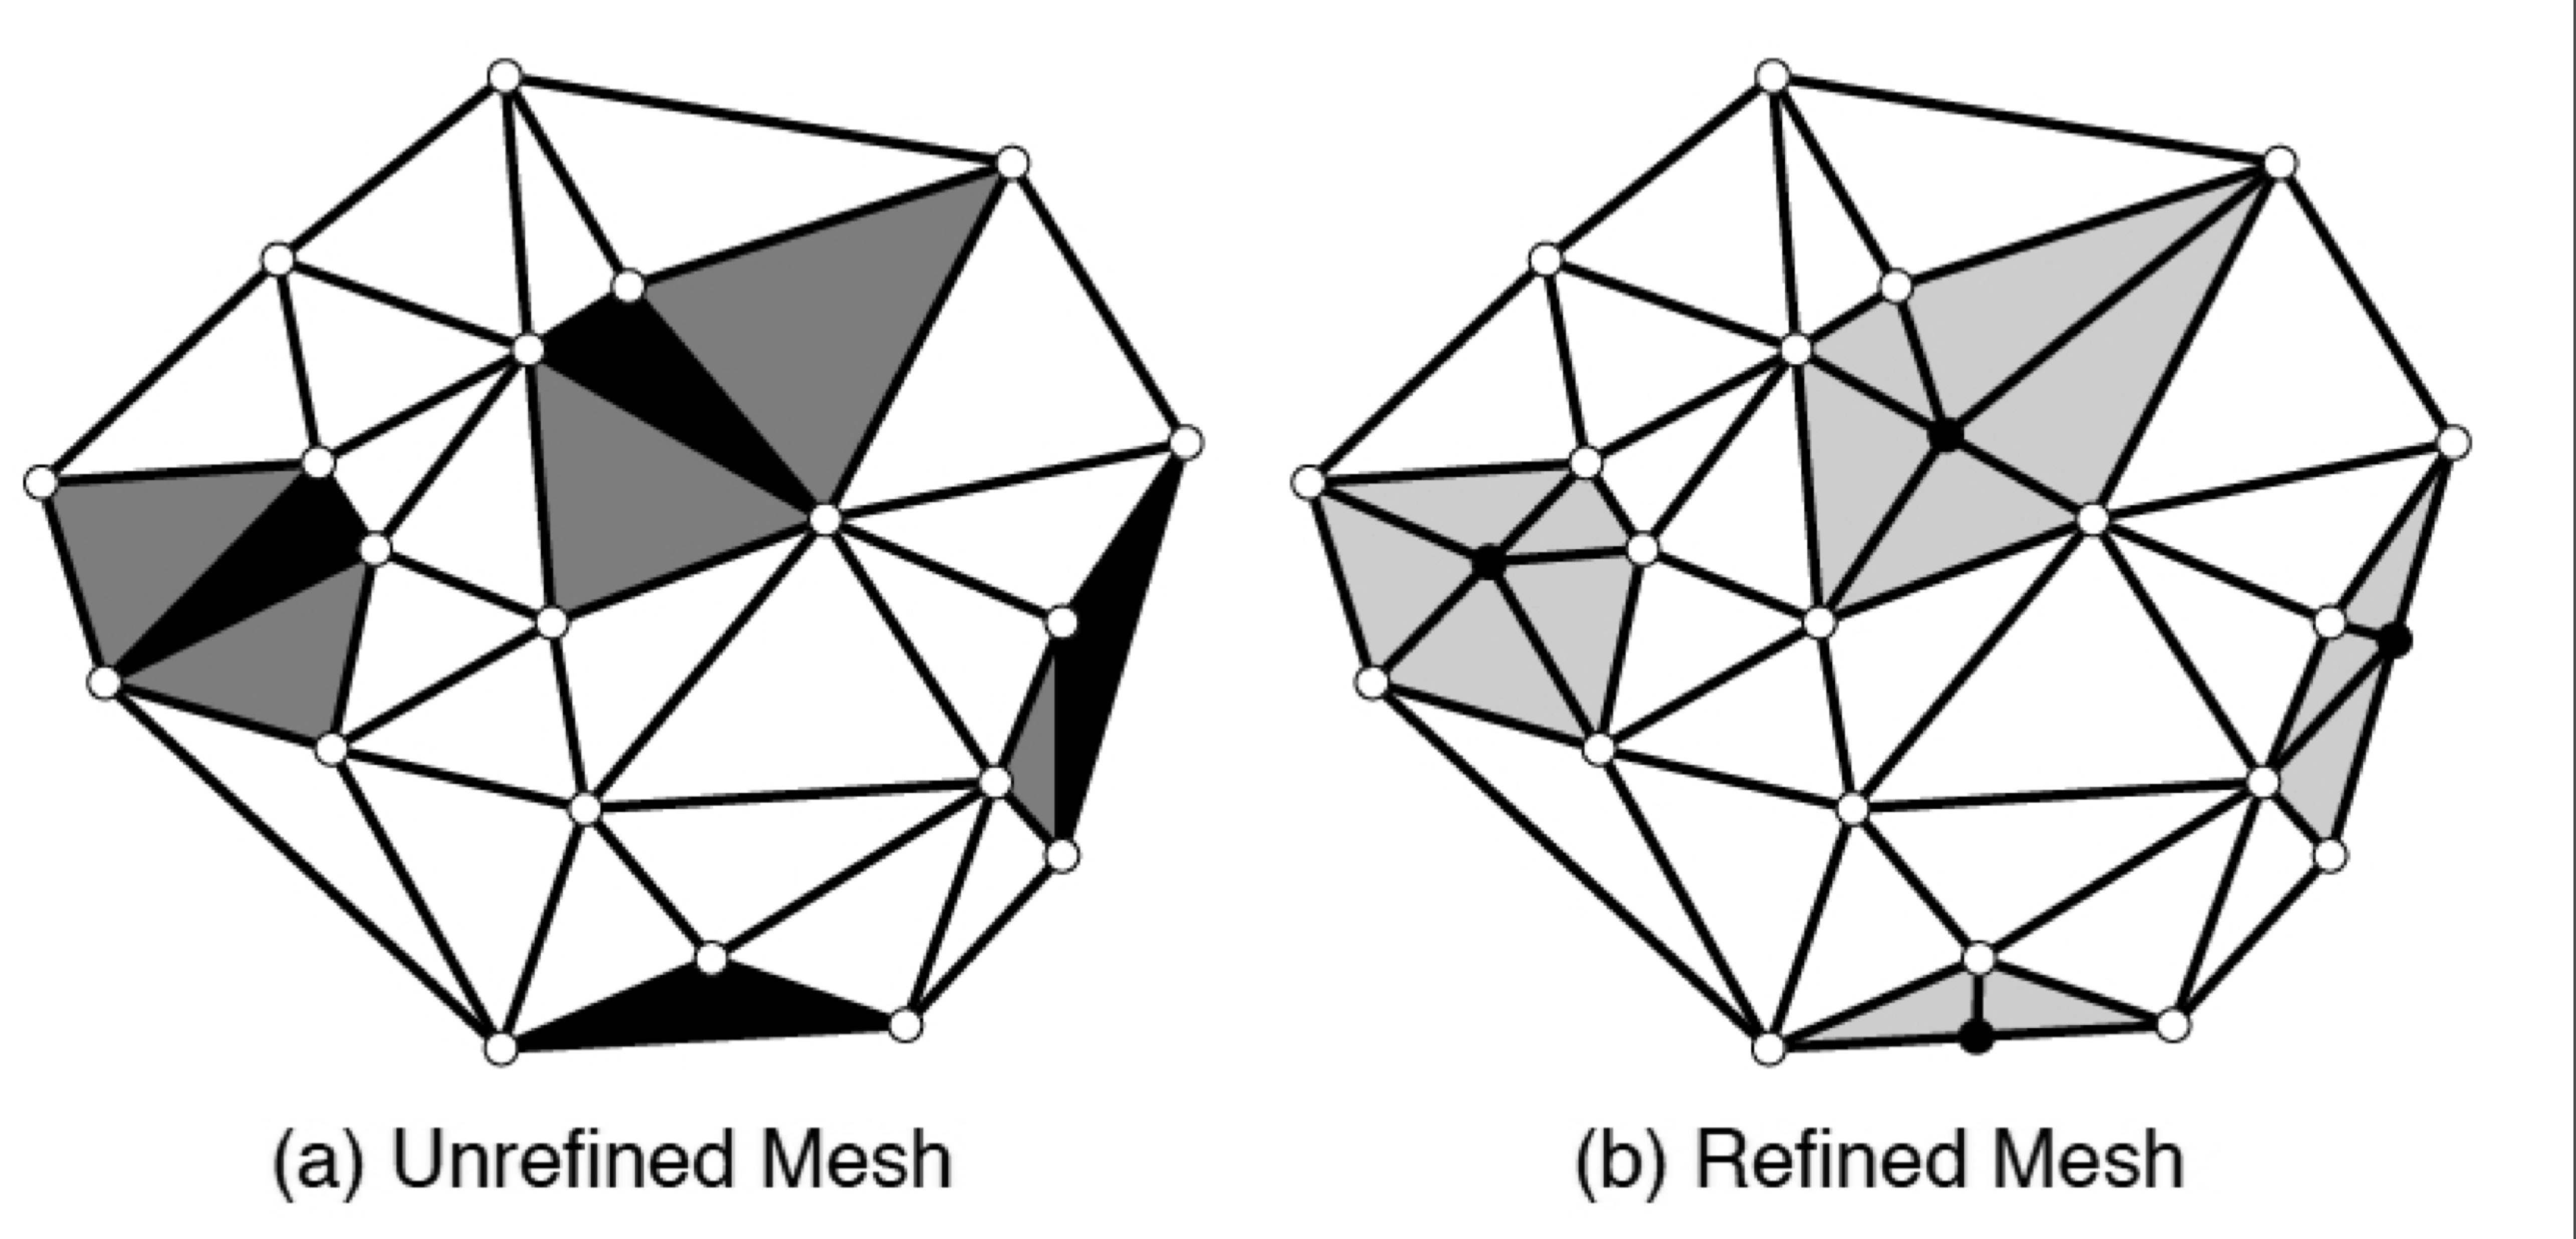
\includegraphics[scale=.15]{graphics-public/delauneypdf}
        \end{quote}
  \caption{A mesh before and after refinement}
  \label{fig:delauney}
\end{figure}

In pseudo-code, this can be implemented as in
figure~\ref{fig:delauney-code}.
\begin{figure}
\begin{displayalgorithm}
Mesh m = /* read in initial mesh */ \\
WorkList wl; \\
wl.add(mesh.badTriangles()); \\
\While { \n{(wl.size() != 0)} } { 
Element e = wl.get(); //get bad triangle \\
if (e no longer in mesh) continue; \\
Cavity c = new Cavity(e); \\
c.expand(); \\
c.retriangulate(); \\
mesh.update(c); \\
wl.add(c.badTriangles()); \\
}
\end{displayalgorithm}
  \caption{Task queue implementation of Delauney refinement}
  \label{fig:delauney-code}
\end{figure}
(This figure and code are to be found in~\cite{Kulkami:howmuch}, 
which also contains a more detailed discussion.)


It is clear that this algorithm is driven by a worklist (or
\indextermbus{task}{queue}) data structure
that has to be shared between all processes. Together with the dynamic
assignment of data to processes, this implies that this type of
\indextermsub{irregular}{parallelism} is suited to shared memory
programming, and is much harder to do with distributed memory.

\index{task!parallelism|)}

\Level 1 {Conveniently parallel computing}

In certain contexts, a simple, often single processor, calculation needs to
be performed on many different inputs.
%
Since the computations have no data dependencies and
need not done in any particular sequence, this is often called
\indexterm{embarassingly parallel} or \indexterm{conveniently
  paralllel} computing.
%
This sort of parallelism can happen at several levels. In examples
such as calculation of the \indexterm{Mandelbrot set} or evaluating
moves in a \indexterm{chess} game, a subroutine-level computation is
invoked for many parameter values.
% 
On a coarser level it can be the case that a simple program needs to
be run for many inputs. In this case, the overall calculation
is referred to as a \indexterm{parameter sweep}. 

\Level 1 {Medium-grain data parallelism}
\label{sec:medium-grain}

The above strict realization of data parallelism assumes that there
are as many processors as data elements. In practice, processors will
have much more memory than that, and the number of data elements is
likely to be far larger than the processor count of even the largest
computers. Therefore, arrays are grouped onto processors in subarrays.
The code then looks like this:
\begin{verbatim}
my_lower_bound = // some processor-dependent number
my_upper_bound = // some processor-dependent number
for (i=my_lower_bound; i<my_upper_bound; i++)
  // the loop body goes here
\end{verbatim}

This model has some characteristics of data parallelism, since the
operation performed is identical on a large number of data items. It
can also be viewed as task parallelism, since each processor executes
a larger section of code, and does not necessarily operate on equal
sized chunks of data.

\Level 1 {Task granularity}
\index{granularity|(}

In the previous subsections we considered different level of finding
parallel work, or different ways of dividing up work so as to find
parallelism. There is another way of looking at this: we define
the \emph{granularity} of a parallel scheme as the amount of work (or
the task size) that a processing element can perform before having to
communicate or synchronize with other processing elements.

In \ac{ILP} we are dealing with very fine-grained parallelism, on the
order of a single instruction or just a few instructions. In true task
parallelism the granularity is much coarser.

The interesting case here is data parallelism, where we have the
freedom to choose the task sizes. On \ac{SIMD} machines we can choose
a granularity of a single instruction, but, as you saw in
section~\ref{sec:medium-grain}, operations can be grouped into
medium-sized tasks. Thus, operations that are data parallel can be
executed on distributed memory clusters, given the right balance
between the number of processors and total problem size.

\begin{exercise}
  Discuss choosing the right granularity for a data parallel operation
  such as averaging on a two-dimensional grid. Show that there is a
  \indexterm{surface-to-volume} effect: the amount of communication is
  of a lower order than the computation. This means that, even if
  communication is much slower than computation, increasing the task
  size will still give a balanced execution.
\end{exercise}

Unfortunately, choosing a large task size to overcome slow
communication may aggrevate another problem: aggregating these
operations may give tasks with varying running time, causing
\indextermbus{load}{unbalance}.  One solution here is to use an
\indexterm{over-decomposition} of the problem: create more tasks then
there are processing elements, and assign multiple tasks to a
processor (or assign tasks dynamically) to even out irregular running
times. Above you already saw \indextermsub{dynamic}{scheduling}; 
an example of \indexterm{over-decomposition} in linear algebra is
discussed in section~\ref{sec:LUscaling}.

\index{granularity|)}
